\section{Ideas}
\subsection{Line search}
Line search in \ref{eqn:update_lsearch} is not working very well. 
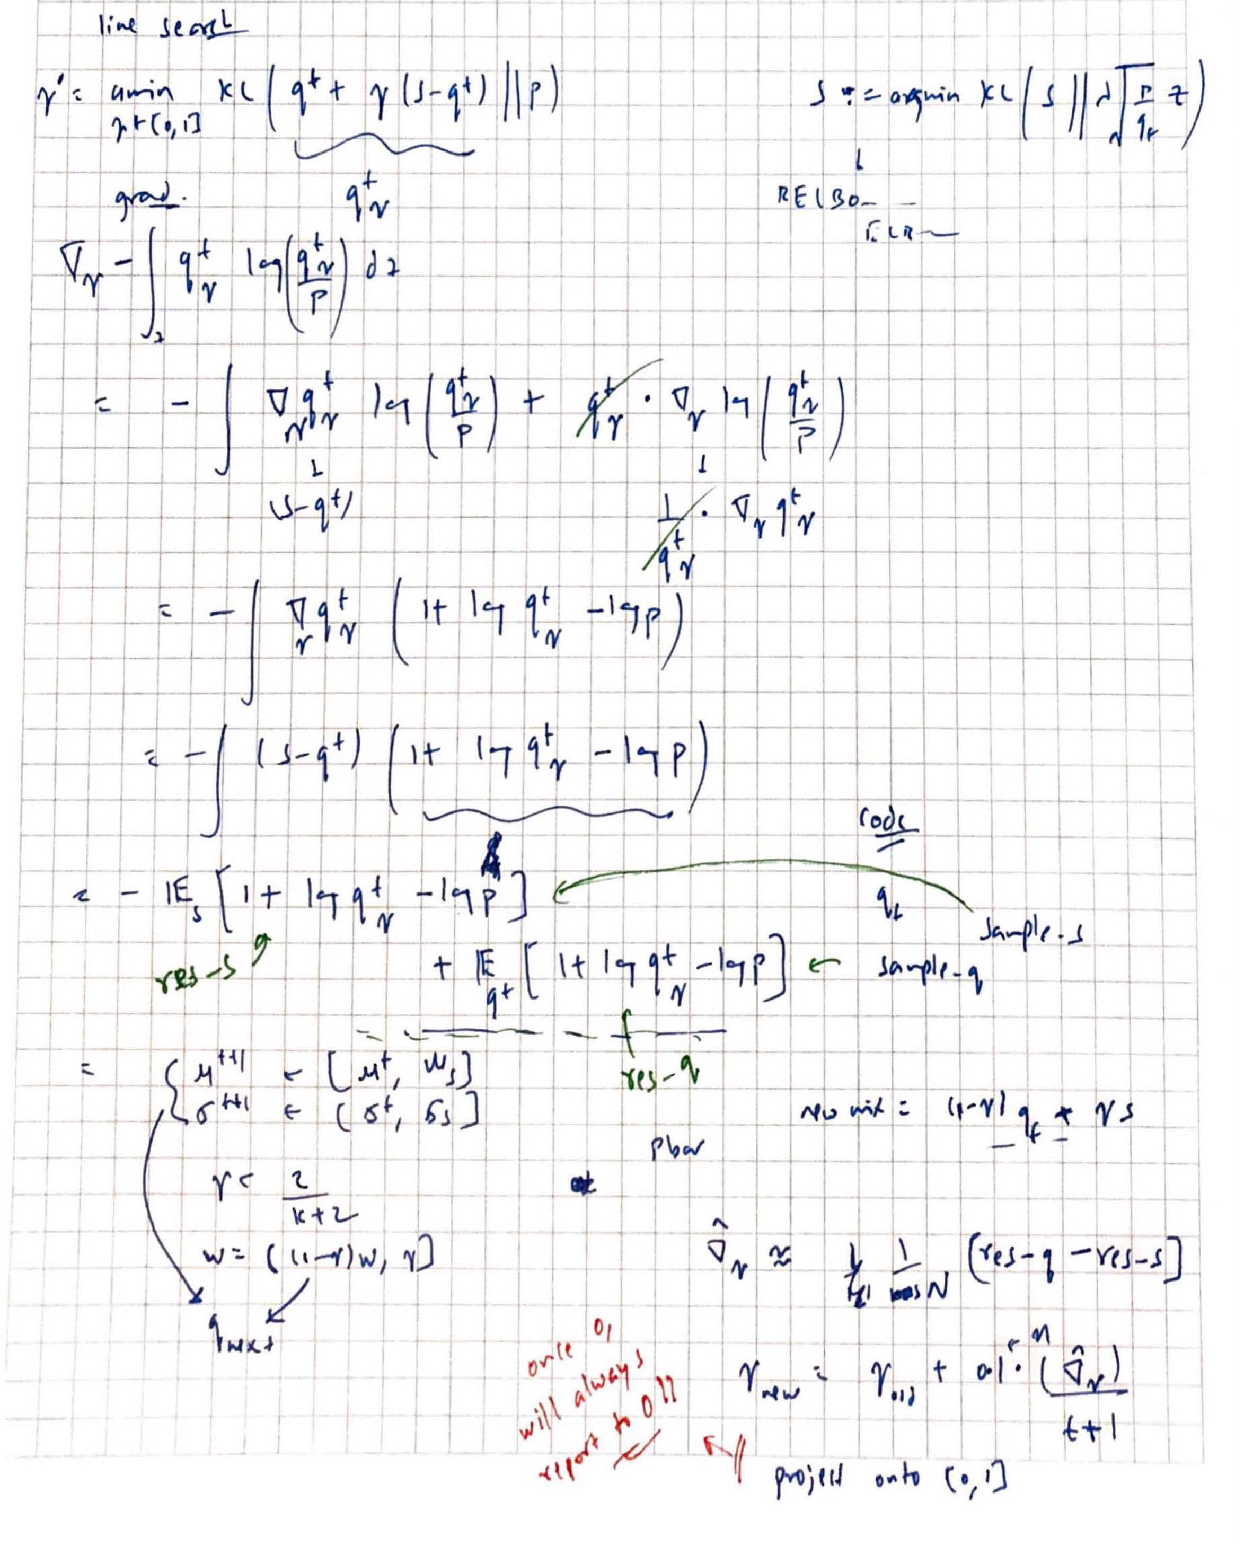
\includepdf{Thesis_notes_Nov_1.pdf}
%\inputminted[firstline=140,lastline=220,mathescape]{python}
%  {../boosting_bbvi/scripts/mixture_model_relbo.py}
\begin{minted}{python}
def line_search_dkl(weights, locs, diags, mu_s, cov_s, x, k):
  """Perform line search for the best step size gamma.

  Uses gradient ascent to find gamma that minimizes
  KL(q_t + gamma (s - q_t) || p)

  Args:
      weights: weights of mixture components of q_t
      locs: means of mixture components of q_t
      diags: deviations of mixture components of q_t
      mu_s: mean for LMO Solution s
      cov_s: cov matrix for LMO solution s
      x: target distribution p
      k: iteration number of Frank-Wolfe
  Returns:
      Computed gamma
  """
  def softmax(v):
      return np.log(1 + np.exp(v))
  # no. of samples to approximate $\nabla_{\gamma}$
  N_samples = 10
  # Create current iter $q_t$
  weights = [weights]
  qt_comps = [
      Normal(
          loc=tf.convert_to_tensor(locs[i]),
          scale=tf.convert_to_tensor(diags[i])) for i in range(len(locs))
  ]
  qt = Mixture(
      cat=Categorical(probs=tf.convert_to_tensor(weights)),
      components=qt_comps,
      sample_shape=N)
  qt = InfiniteMixtureScipy(stats.multivariate_normal)
  qt.weights = weights[0]
  qt.params = list(
      zip([[l] for l in locs], [[softmax(np.dot(d, d))] for d in diags]))
  # samples from $q_t$
  sample_q = qt.sample_n(N_samples)
  # create and sample from s
  s = stats.multivariate_normal([mu_s],
                                np.dot(np.array([cov_s]), np.array([cov_s])))
  sample_s = s.rvs(N_samples)
  # $q_{t+1}$ is mixture of $q_t$ and s with weights $(1 - \gamma)$ and $\gamma$
  # Set its corresponding parameters and weights
  new_locs = copy.copy(locs)
  new_diags = copy.copy(diags)
  new_locs.append([mu_s])
  new_diags.append([cov_s])
  # initialize $\gamma$
  gamma = 2. / (k + 2.)
  # no. steps of gradient ascent
  n_steps = 10
  prog_bar = ed.util.Progbar(n_steps)
  for it in range(n_steps):
  print("line_search iter %d, %.5f" % (it, gamma))
  new_weights = copy.copy(weights)
  new_weights[0] = [(1. - gamma) * w for w in new_weights[0]]
  new_weights[0].append(gamma)
  # create $q_{t + 1}^{\gamma}$
  q_next = InfiniteMixtureScipy(stats.multivariate_normal)
  q_next.weights = new_weights[0]
  q_next.params = list(
  zip([[l] for l in new_locs], [[np.dot(d, d)] for d in new_diags]))
  # Computes $\mathbb{E}[...] \propto \sum_{v}{\log p - \log q_{t + 1}^{\gamma}}$
  def px_qx_ratio_log_prob(v):
  Lambda = 1.
  ret = x.log_prob([v]).eval()[0] - q_next.log_prob(v)
  ret /= Lambda
  return ret
  # Samples w.r.t s
  rez_s = [
  px_qx_ratio_log_prob(sample_s[ss]) for ss in range(len(sample_s))
  ]
  # Samples w.r.t $q_{t+1}$
  rez_q = [
  px_qx_ratio_log_prob(sample_q[ss]) for ss in range(len(sample_q))
  ]
  # Gradient ascent step, step size decreasing as $\frac{1}{it + 1}$
  gamma = gamma + 0.1 * (sum(rez_s) - sum(rez_q)) / (N_samples *
  (it + 1.))
  # Projecting it back to [0, 1], too small range?
  # FIXME(sauravshekhar) if projected to 0, all iterations will be same?
  if gamma >= 1 or gamma <= 0:
  gamma = max(min(gamma, 1.), 0.)
  break
  return gamma
\end{minted}
\mypar{changes for measuring variance of $\EEE{s}{\cdot}$ and $\EEE{q_{t+1}^{\gamma}}{\cdot}$}
\begin{minted}{python}
    ...
    grad_gamma = []
    for it in range(n_steps):
    ...
    # Samples w.r.t s
    rez_s = np.asarray([
        px_qx_ratio_log_prob(sample_s[ss]) for ss in range(len(sample_s))
    ])
    # Samples w.r.t $q_{t+1}$
    rez_q = np.asarray([
        px_qx_ratio_log_prob(sample_q[ss]) for ss in range(len(sample_q))
    ])
    grad_gamma.append({'E_s': rez_s, 'E_q': rez_q, 'gamma': gamma})
    ...
    # Write grad_gamma to outdir/line_search_samples_<n_samples>.npy.<fw_iter>
\end{minted}
\mypar{Metrics on original version}
\begin{figure}[h] \label{fig:gamma}
  \centering
  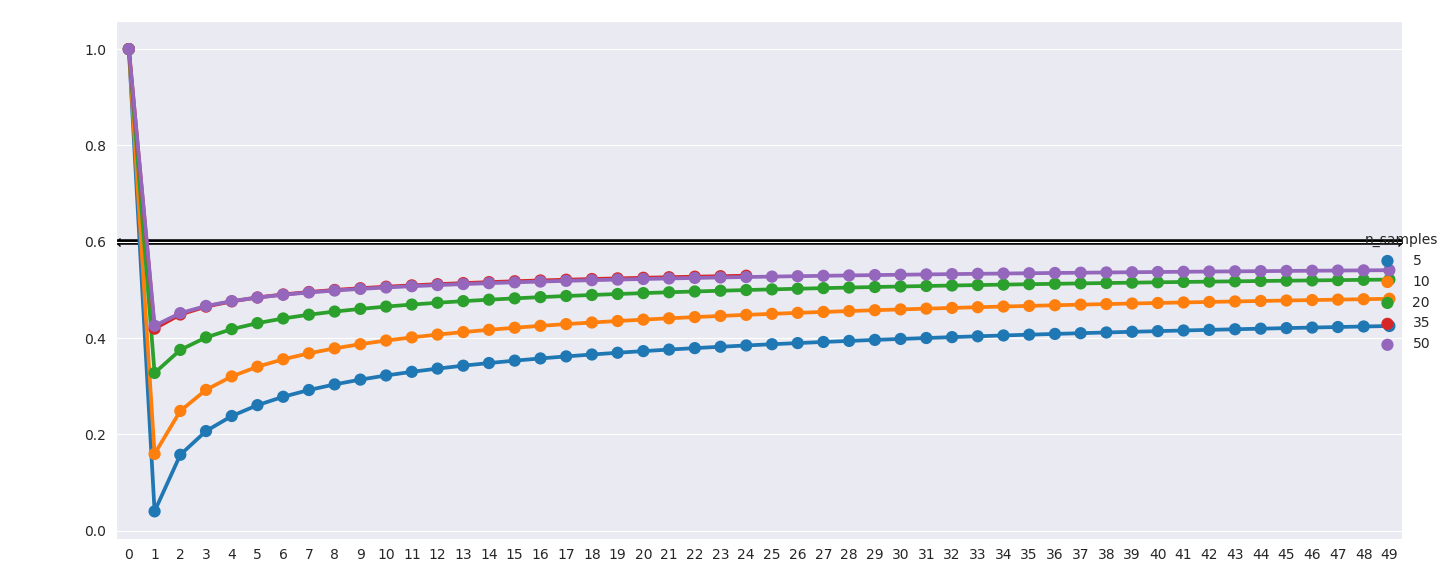
\includegraphics[width=0.9\textwidth]{plots/test_gamma.png}
  \caption{gamma with iterations for different n\_samples}
\end{figure}
\begin{figure}[h] \label{fig:es}
  \centering
  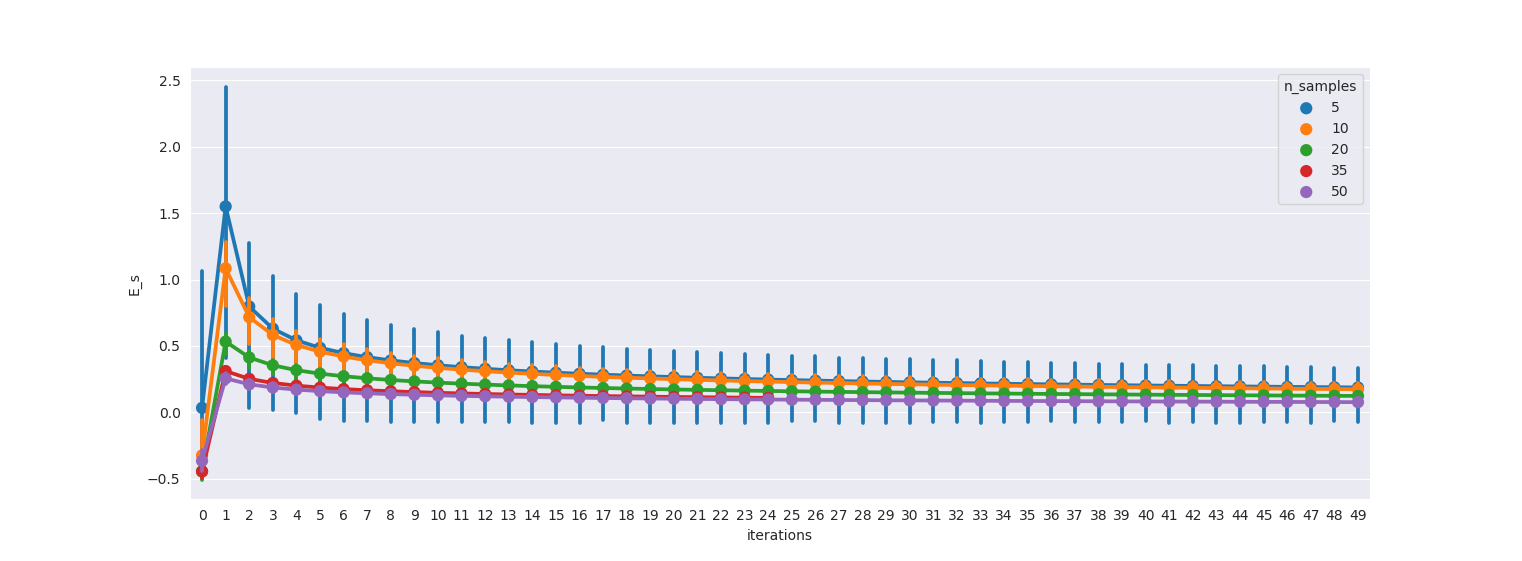
\includegraphics[width=0.9\textwidth]{plots/test_e_s.png}
  \caption{$E_s$ with different n\_samples}
\end{figure}
\begin{figure}[h] \label{fig:eq}
  \centering
  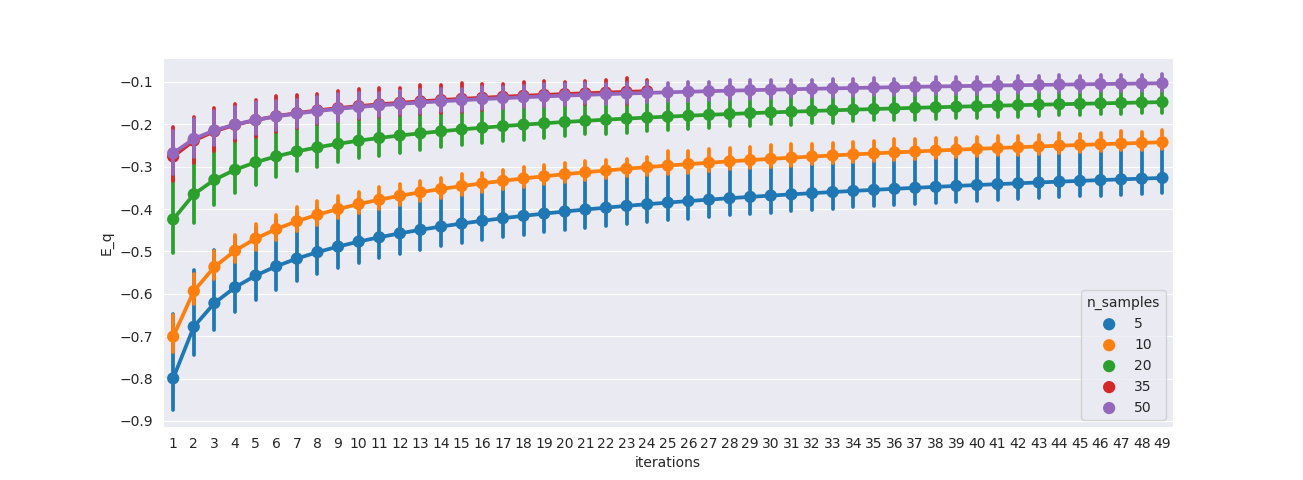
\includegraphics[width=0.9\textwidth]{plots/test_e_q.png}
  \caption{$E_q$ with different n\_samples}
  \small{\comment{\ref{fig:eq} begins with iter 1 as iter 0 has very high variance}}
\end{figure}

\subsection{Measuring smoothness}
\INPROGRESS
Computing optimal $\gamma$ directly
from eqn 1 of \cite{pedregosa2018step}
\begin{align*}
  f(\bx_{t+1}) &\leq f(\bx_t) + \gamma \langle \grad f(\bx_t), \bs_t - \bx_t \rangle 
  + \frac{\gamma^2}{2}L_t ||\bs_t - \bx_t||^2 \\
  \Rightarrow L_t &\geq \frac{f(\bx_{t+1}) - f(\bx_t) 
  + \gamma \langle \grad f(\bx_t), \bs_t - \bx_t \rangle}
  {\frac{\gamma^2}{2}||\bs_t - \bx_t||^2}  \\
                  &\frac{f(\bx_{t+1}) - f(\bx_t) 
                  + \gamma \langle \grad f(\bx_t), \bs_t - \bx_t \rangle}
                  {\frac{\gamma^2}{2} \red{\kl{s_t || q_t}}}  \\
    \langle f, g \rangle &= \int f(\theta) f(\theta) d\theta 
    \text{  \comment{//functional dot product}}\\
  \end{align*}
  \mypar{Code changes}
  \begin{minted}{python}
  def kl(mu_q, std_q, mu_p, std_p):
    ...

  def func_dot_product():
    ...
  \end{minted}

  \subsection{Other optimization algorithm}
  \TODO
  As shown in link \ref{web:cmu}, Frank-Wolfe converges slower than Projected 
  Gradient Descent in Practice. See \cite{locatello2017boosting} to see why we use
  FW and if it can be replaced. (will have to derive new convergence proofs and
  boosting won't be as integrated into the optimization algorithm as before).

